\chapter{High Doping Concentrations in Nanowires}
\label{sec:high}

This chapter will discuss the concentration of dopants incorporated into ion irradiated nanowires. Some of the first results were published in reference \cite{johannes_enhanced_2014}. The simulations and experiments presented in this chapter where all performed on $Mn^+$ irradiated $ZnO$ nanowires, however the effects are easily applied to other material combinations.

\section{Doping and Sputtering}

With \emph{iradiana} the distribution of the places where the ions come to rest gives the profile of the concentration of dopants per fluence. Locally the concentration, in [$atoms/cm^{3}$], increases a certain amount per fluence, in [$ions/cm^{2}$], leading to the somewhat awkward unit of for the doping efficacy, $[(atoms/cm^{3})/(ions/cm^{2})]$.
An example of simulation results is shown in figure \ref{iradinacrossection}a for the irradiation of a $ZnO$ nanowire with $175\,keV\,Mn^+$. The ions enter the $y-z$ plane at random locations an an angle of $45^\circ$ to the $z$-axis, which is periodically continued outside the plane of the image. It is clear, that a homogeneous doping profile is not easy to obtain for the irradiation of a nanowire from one side. As with the creation of a box profile in bulk irradiation, multiple irradiation steps with varying energy are required. Note that $175\,keV$ ion energy are obviously not enough to permeate the whole nanowire diameter of $200\,nm$, so that a higher ion energy is required. Rotating the nanowire under the ion beam is a much easier way of increasing homogeneity of the doping profile. Figure \ref{iradinacrossection}b shows the local dopant incorporation efficacy for the rotation of the profile show in \ref{iradinacrossection}a. Irradiation with a single, relatively low ion energy produces a homogeneous doping profile. 
  
\begin{figure}
	\centering
		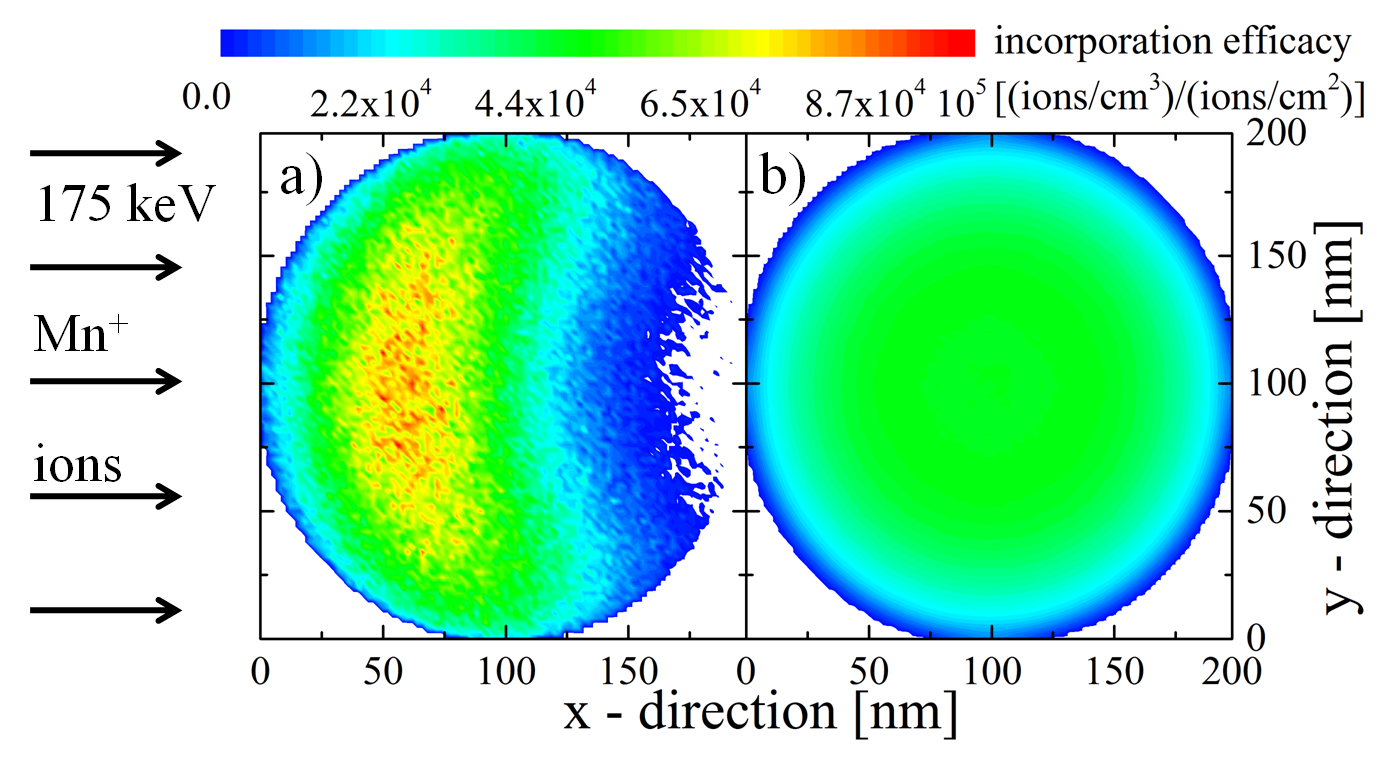
\includegraphics[width=.8\textwidth]{images/iradinacrosssection.png}
	\caption{a) Color plot of the increase in concentration per fluence for the irradiation of a $ZnO$ nanowire with $175\,keV\,Mn^+$ ions at an angle of $45^\circ$ to the $z$-axis. The energy was selected so that the rotation of this profile produces a radially homogeneous dopant distribution, as shown in b). The mean dopant incorporation efficacy is $3.4\cdot10^4\,(atoms/cm^3)/(ion/cm^2)$.}
	\label{iradinacrossection}
\end{figure} 

As lower energy ions have lower ranges, there are fewer paths that cause the ion to leave the nanowire, particularly in the forward direction. Therefore, the first advantage of decreasing the ion energy is that the doping efficacy is larger for lower ion energies, so a lower irradiation fluence is required to achieve doping at a desired level. Furthermore, lower ion energy impacts also produce less damage in the irradiated matrix. Together with an optimal irradiation temperature the rotated irradiation was utilized to improve the magnetic properties of $Mn^+$ irradiated $GaAs$ nanowires \cite{borschel_new_2011,paschoal_hopping_2012,borschel_ion-solid_2012,kumar_magnetic_2013,paschoal_magnetoresistance_2014}. 

The assumption underlying the doping efficacy and using it to calculate the required fluence for a desired doping concentration is that the concentration increases linearly with the irradiated fluence. This is only true in the absence of sputtering. In figure \ref{iradinacrossection}b the outermost layer of the nanowire has a lower dopant incorporation efficacy than the rest of the wire volume. Since the sputtered atoms predominantly originate from this outer layer, the matrix of the nanowire is eroded at the same time as dopants are incorporated. Sputtering therefore leads to a non-linear increase in the concentration of dopants with the irradiated fluence.

\section{Pseudo-dynamic simulation}

For the direct simulation of the effect of sputtering on the incorporation of dopants into nanowires a dynamic simulation program which also considers the three dimensional geometry of the target is required. However, with results from static simulations for varying diameters, a pseudo-dynamic study can be conceived. The sputter yield is dependent on the nanowire radius and the ion energy as shown in \ref{sputterincorporate}a. The dependency is discussed in detail in the previous chapter \ref{sec:simsputering}. Likewise the incorporation efficacy plotted in \ref{sputterincorporate}b is also dependent on the nanowire radius and the ion energy. For increasing ion energy the efficacy is monotonically decreasing, as the probability of the ion to leave the nanostructure rises together with the ion range. For moderate, fixed ion energies the probability of an ion to stay in the nanostructure increases with increasing diameter, so that at first the efficacy also increases with increasing diameter. For large diameters this effect is overcompensated by a stronger dilution of the dopants in the volume of the nanowire which increases as the square of the diameter. For a fixed energy the efficacy has a maximum at a \TODO{SRIM range}
 

\begin{figure}
	\centering
		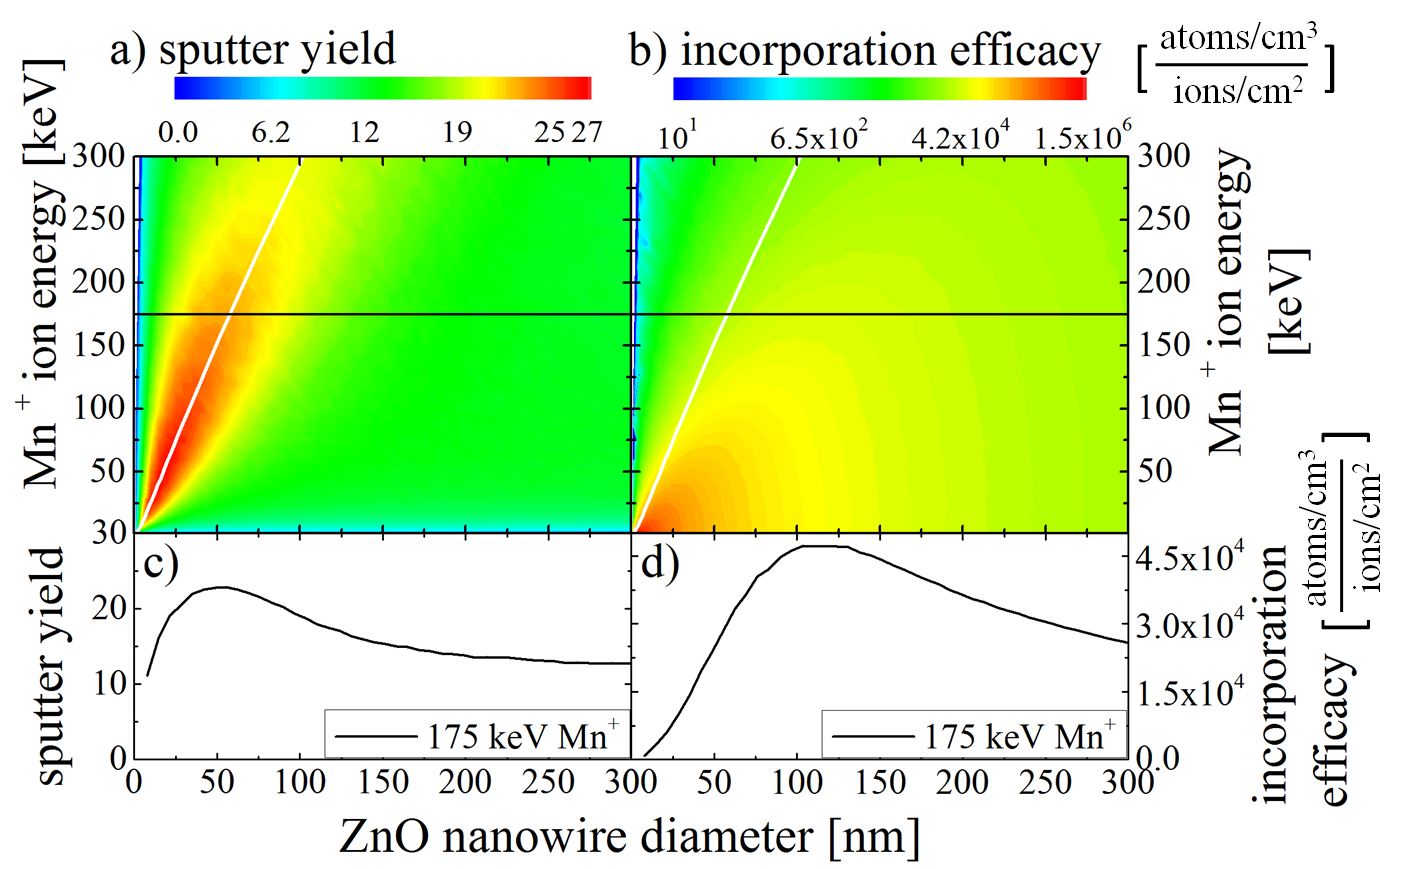
\includegraphics[width=.85\textwidth]{images/sputterincorporate.png}
	\caption{a) Sputter yield for the irradiation with $Mn^+$ of ZnO nanowires with varying diameters an ion energies. From the same simulations the dopant incorporation efficacy was determined and plotted in b).}
	\label{sputterincorporate}
\end{figure} 


\section{Results from optimal irradiation conditions}

\section{Discussion of relevant effects}

redeposition from substrate (numeric Simulation)

shadowing with old results

\subsubsection{Discussion}